% !TEX root = ../agglo_clust_review.tex

\section{Introduction}
%On possible selling story could be: currently many of the successful proposal-free instance segmentation methods rely on a final clustering step on a grid-graph with both short and long-range connections. So it is worth to study this problem in more details. 

\emph{Instance segmentation} is a task of computer vision consisting in assigning each pixel of an image to an object instance \TODO{REF}. The most success in instance segmentation (IS) has been achieved by applying deep learning [REF]. There are two main types of deep learning approaches to IS: proposal-based and proposal-free methods. Proposal-based methods consist of two steps: object detection, for example by finding bounding boxes around the objects, and assigning pixels to the detected objects \TODO{REF}. Although these approaches have proven to be highly successful in instance segmentation competitions like MS COCO \cite{lin2014microsoft}, Pascal VOC2012 \cite{everingham2010pascal} and CityScapes \cite{cordts2016cityscapes}, they are not applicable to certain types of data, for example microscopy images of neurons \TODO{cremi, isbi}, where objects are not approximated well by bounding boxes. 
% More motivation: They are at the same time limited by the quality of the object detection routine, which is hard to train on small datasets (but no ref for this)
Proposal-free methods perform IS by directly predicting pixel features and then using a clustering algorithm for grouping pixels into object instances \TODO{REF}. In this paper, we focus on a proposal-free method, where a Convolutional Neural Network (CNN) predicts affinities representing how likely it is for pairs of pixels to belong to the same instance. Recently, this approach was used in \cite{liu2018affinity} to achieve a performance comparable to the proposal-based methods on the Cityscapes dataset and in \cite{wolf2018mutex} to achieve state-of-the-art results in a competitive neuron segmentation challenge. 

The output of the CNN can be represented as a weighted grid graph such that each node represents a pixel of the image and the weights of the edges define interactions between the pixels. A graph clustering algorithm is then applied to cluster pixels into instances. The majority of clustering methods work with positive edge weights only, representing attractive interactions between the nodes. These methods require the user to specify the desired numbers of segments or a termination criterion (as in spectral clustering or iterated normalized cuts) or even a stronger version of supervision in terms of seeds (as in seeded watershed or random walker).  

A popular method for graph clustering is hierarchical clustering (HC) which creates an hierarchy of clusters. Agglomerative HC is a bottom-up approach starting with each node assigned to its own cluster and incrementally merging clusters while moving up the hierarchy REF?. This method requires the user to choose a level in the cluster hierarchy defining the desired output clustering. 

Other clustering methods work with so-called \emph{signed graphs}, which include both positive and negative edge weights corresponding to attraction and repulsion between pixels [REF]. The advantage of using signed graphs is that balancing attraction and repulsion allows us to perform the clustering without defining additional parameters. For small problems, this can be done optimally by solving the so-called \emph{multicut optimization problem} or \emph{correlation clustering}; however, this problem is NP-hard and thus not scalable [REF]. Other recently algorithms applicable to signed graphs are greedy approximations of the multicut pro



As to our knowledge, related work applies HC to graphs with positive weights only \TODO{REF}. 

\begin{itemize}



\item \emph{Possible intro about aggl. clustering:} \UPDATE{Hierarchical, agglomerative clustering is an important and well-established technique in unsupervised machine learning. Agglomerative clustering schemes start from the partition of the data set into singleton nodes and merge step by step the current pair of mutually closest nodes into a new node until there is one final node left, which comprises the entire data set. Various clustering schemes share this procedure as a common definition, but differ in the way in which the measure of inter-cluster dissimilarity is updated after each step. } %\cite{mullner2011modern}



\item \emph{Other possible intro:} Many problems in computer vision involve clustering. Partitional clustering, such as k-means [1], determines all clusters at once, while agglomerative clustering [1] begins with a large number of small clusters, and iteratively selects two clusters with the largest affinity under some measures to merge, until some stopping condition is reached. Ag- glomerative clustering has been studied for more than half a century, and used in many applications [1], because it is conceptually simple and produces an informative hierar- chical structure of clusters. % FROM https://arxiv.org/pdf/1208.5092.pdf#page14

\item Get more specific about graph (we do not cluster points in a space, but we cluster vertices with specified neighbors and interactions given by edges). 

\item HC is a popular graph partitioning algorithm. Why: more efficient than divisive approaches and graph cuts; does not usually require to specify the final number of clusters (e.g. spectral clustering) or seed nodes (e.g. watershed, random walker). \UPDATE{And if the graph is not dense, HC algorithms scale up well with complexity}

\item Motivation 1:

\begin{itemize}

\item all HC methods only talk about positive edge weights, but it is actually easy to generalize them for negative and attractive edges. 
\item The standard version of HC is good for building hierarchy but problem with hierarchical merge-trees is how to choose one single threshold. Choose one single fixed density level. Ideally we would like to be able to cut the tree at different places to select our clusters.
\item An important line of research is based on the observation that superior partitionings are obtained when the graph has both attractive and repulsive edges. Solutions that optimally balance attraction and repulsion do not require external stopping criteria such as predefined number of regions or seeds. This generalization leads to the NP-hard problem of correlation clustering or (synonymous) multicut (MC) partitioning. \emph{Alternative:} multicut / correlation clustering partitions vertices with both attractive and repulsive interactions encoded into the edges of a graph. Multicut has the great advantage that a “natural” partitioning of a graph can be found, without needing to specify a desired number of clusters, or a termination criterion, or one seed per region. Its great drawback is that its optimization is NP-hard.

\item Contributions: (and mention introductory Figure)
\begin{itemize}
\item We generalize the hierarchical agglomerative clustering framework to graphs with positive and negative edge attributes
\item We review both standard hierarchical clustering algorithms and signed graph partitioning algorithms by showing how they can be described in this simplified framework (and as special cases of the general algorithm presented in Sec. \ref{sec:algorithm})
\item we introduce and test new variations of these algorithms for signed graphs
\end{itemize}
\end{itemize}

\item Motivation 2:
\begin{itemize}
\item HC has been always really popular in computer vision: \emph{Instance segmentation} is a task of computer vision that involves the detection of all objects in an image by performing pixel-level segmentation of each instance.   
\item Since conventional unsigned graph agglomerative clustering algorithms, such as the well-known linkage methods [1], usually are quite sensitive to noise and outliers [1] (As their affinities are directly computed using pairwise distances between samples), most methods were based on multi-step pipelines first predicting superpixels (to reduce noise).
\item These methods are still commonly used for specific instance segmentation applications: connectomics, build merge-tree 
 %https://arxiv.org/pdf/1208.5092.pdf
\item still commonly used for building merge-trees, give recent examples in connectomics (Sebastian Seung, etc...) % https://arxiv.org/abs/1608.04051
\item Graph clustering algorithms recently gained more and more popularity with the advent of deep-learning and its application to instance segmentation
\item Deep convolutional neural nets (CNNs) has been successfully applied to a wide range of tasks of computer vision and pixel-level image understanding, such as \UPDATE{boundary detection \cite{arbelaez2011contour,xie2015holistically,maninis2018convolutional}, semantic segmentation \cite{long2015fully,chen2018deeplab,kong2018recurrent}, optical flow \cite{weinzaepfel2013deepflow,dosovitskiy2015flownet}, and pose estimation \cite{wei2016convolutional,cao2017realtime}.}
% \SOURCE{\cite{kong2018recurrent}}

\item Currently there are two successful approaches used for proposal-free bottom-up instance segmentation: the first ones predict associative pixel embedding vectors, where the goal is to have a CNN predicting embedding vectors that are similar only for pixels in the same instance \cite{kong2018recurrent,fathi2017semantic,newell2017associative,de2017semantic}; in the second type of approaches, for every pixel a set of neighboring pixels is fixed  (not necesarelly limited to the direct neighbors) and a CNN then predicts affinities, that represent how likely it is for each of neighboring pixels to be in the same instance \cite{liu2018affinity,wolf2018mutex,xie2015holistically}

\item Both approaches requires a final clustering algorithm to output the final instance segmentation 

 and we can define a grid graph, where each vertex represents a pixel, with short- and long-range edge connections 

 and find the final instance segmentation by using a graph clustering algorithm.

\item GMIS achieved 
comparable results to methods based on object 
proposal like Mask-R-CNN on natural images 
(Cityscapes); MWS achieved SOA results on a 
biological images (ISBI)

\item Out contributions:

\begin{itemize}
 \item we compare different types of agglomeration clustering on a pixel grid graph with short and long-range connections, focusing on aspects like efficieny, robustness (and quality of the final clustering in terms of multicut energy) \textbf{Comparison paper}
 \item \textit{if we get good scores on CREMI dataset}: we show that also on neuro-data it is worth to skip the hand-crafted superpixel step and compute the final segmentation directly from the CNN affinities (MWS already showed it on the ISBI dataset): main selling point is again the almost-parameter free feature of the method
\end{itemize}
\end{itemize}
\end{itemize}


More details about instance segmentation (move to related work)
\begin{itemize}


\item 
\item Many recent successful methods for instance segmentation %, usually named \emph{proposal-based methods}, 
 use heuristic approaches that start from the classical computer vision task of \emph{object detection}, where the goal is to localize each objects using a bounding box, and then predict both a pixel-level mask of each instance and a semantic label (classify the objects in the bounding box). \TODO{Is it really general enough as a description...?} \cite{yang2012layered,ladicky2010and,hariharan2014simultaneous,chen2015multi,dai2016instance,liang2016reversible,he2017mask}
\item While effective, these approaches are \UPDATE{somewhat unsatisfying (copy/paste, change: present some faults)} because:
\begin{itemize}
\item they rely on the object detector and non-maximum suppression heuristics to count how many instances are present in the image, 
\item they tend to underperform in cluttered scenes, since instance assignment is often carried out independently for each detection; 
\item they are not usable for wiry or articulated objects (e.g. in the field of connectomics and neuron segmenation from electron microscopy images) 
\item their architecture do not usually prevent a pixel to be shared between multiple instances
\item they do not scale up well since each proposal has to be singularly processed by the CNN. 
% \item (difficult to train in an end-to-end manner: interface between instance segmentation and detection is non-differentiable)
% \item (architecture is complex and hard to tune and “debug”...?)
\end{itemize}

\item Currently there are two successful approaches used for proposal-free (make brief intro) instance segmentation: the first ones predict associative pixel embedding vectors, where the goal is to have a CNN predicting embedding vectors that are similar only for pixels in the same instance \cite{kong2018recurrent,fathi2017semantic,newell2017associative,de2017semantic}; in the second type of approaches, for every pixel a set of neighboring pixels is fixed  (not necesarelly limited to the direct neighbors) and a CNN then predicts affinities, that represent how likely it is for each of neighboring pixels to be in the same instance \cite{liu2018affinity,wolf2018mutex,xie2015holistically}

\item Both approaches requires a final clustering algorithm to output the final instance segmentation 

 and we can define a grid graph, where each vertex represents a pixel, with short- and long-range edge connections 

 and find the final instance segmentation by using a graph clustering algorithm.

\item Recent work (\cite{wolf2018mutex}, more...) shows that it is better to use \textbf{repulsion and attraction} (directly predict it with the classifier, no need to define seeds or to fix a threshold given an hierarchy of clusters)
\item solving correlation clustering problem (multicut) is too expensive for this application (even using recently proposed heuristics)
\item our contributions:
\begin{itemize}
\item we propose a unified and simple formalization of Agglomerative Clustering and show how many of the recently proposed methods can be seen as special cases (focusing in particular on signed graphs) (\textbf{review and comparison paper})
\item new clustering algorithms on signed graphs


\end{itemize}
\item on other datasets (connectomics) many methods are based on multi-step pipelines first predicting superpixels


\end{itemize}


\begin{figure}[t]
\centering
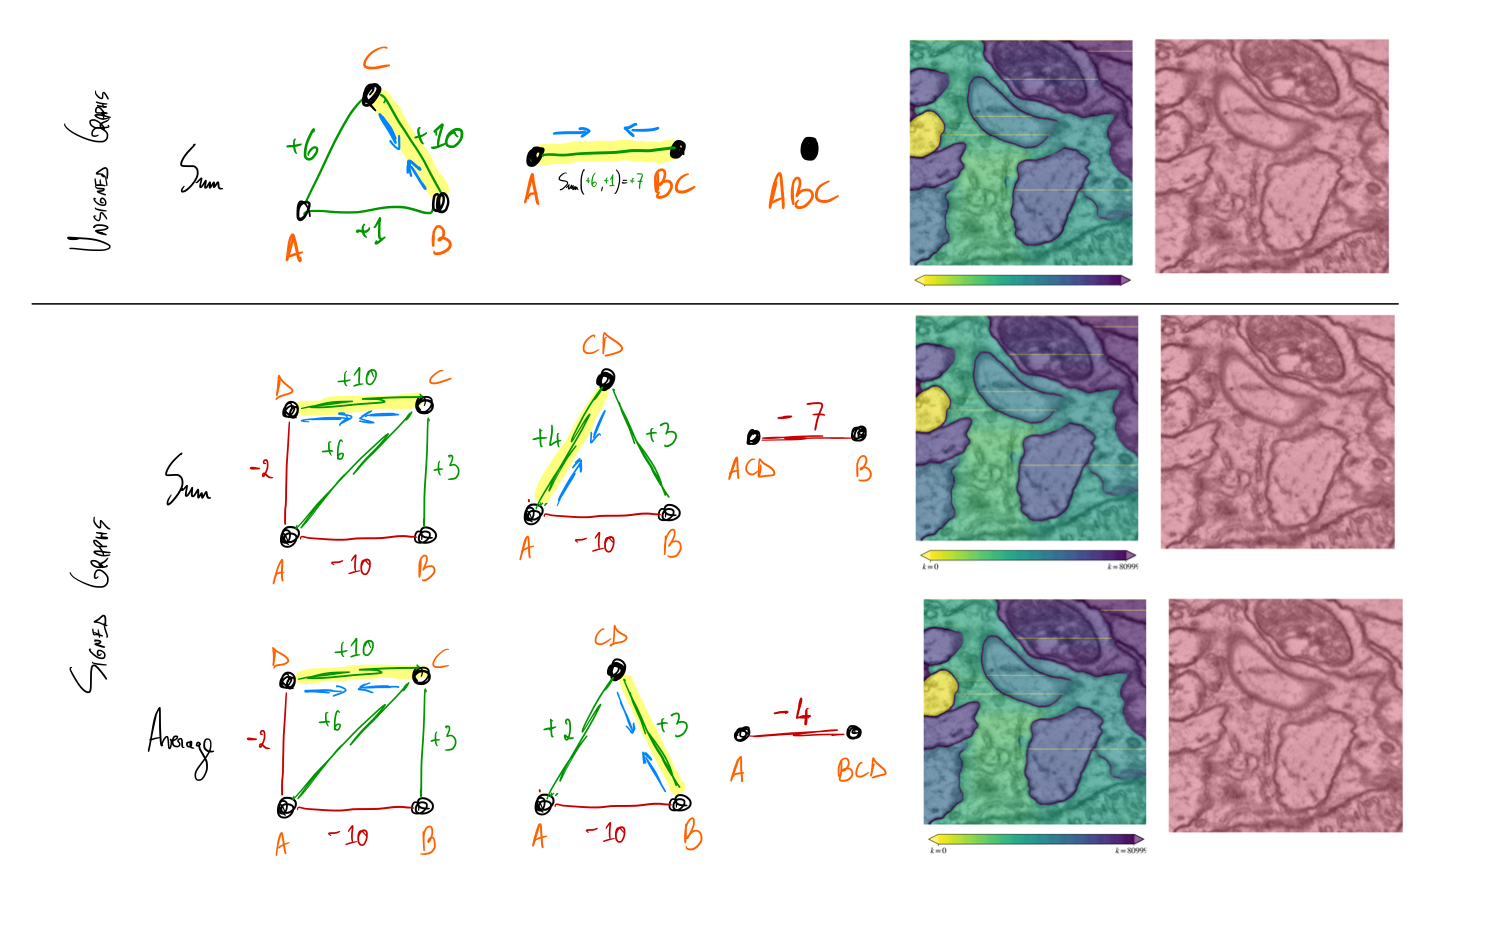
\includegraphics[width=\textwidth,trim=0.4in 1.2in 0.in 0.05in,clip]{./figs/intro_image.jpg} % left bottom right top
\caption{\small 
Intro image: explain algorithm, main ideas and contributions
\label{fig:intro_figure}}
\end{figure}
